\documentclass[9pt,dvipdfmx,a4paper]{jsarticle}

\usepackage{amsmath,amssymb}
\usepackage{bm}
\usepackage[dvipdfmx]{graphicx}
\usepackage{physics} % http://mirrors.ibiblio.org/CTAN/macros/latex/contrib/physics/physics.pdf
\usepackage{siunitx} %SI単位を楽に出力
\usepackage{mathtools} %環境の追加
\usepackage{circuitikz} %電気回路をtex中で書く
% \usepackage{caption} %番号なしキャプションを書く
% \usepackage{cancel} %式中に斜線を入れる
% \usepackage{tensor} %テンソルの添え字を書く
% \usepackage{tikz} %図を書く
% \usepackage{ascmac} %四角い枠の中に文章を書く
% \usepackage{float} %figureで[hbp]オプションを使う
% \usepackage{hyperref}  \usepackage{pxjahyper} %ハイパーリンクをつかう
% \usepackage{tablefootnote} %表中に注釈をいれる
% \usepackage[thicklines]{cancel} %数式中の取り消し線
\usepackage[version=4]{mhchem} %化学式の入力
\usepackage{pdfpages}
\usepackage{wrapfig} %文章の回り込み
\usepackage[subrefformat=parens]{subcaption} %(a)図のようにすることができるやつ
\usepackage{here}
\usepackage{mathrsfs} % フォントの追加
\usepackage{url} % url を入れる
\usepackage[margin=15mm]{geometry} %余白の削除
\usepackage{tcolorbox}

\renewcommand{\abstractname}{Abstract}

\usepackage{fancyhdr}
\pagestyle{fancy}
\lhead{応用物理学実験:熱測定で見る相転移}
\rhead{\bf\thepage}
\cfoot{}

\graphicspath{{./image/}}

\begin{document}

%出力したpdfを表紙にするとき
% \includepdf[pages=1,noautoscale=false]{cover.pdf}
% \newpage

%texで表紙を書くとき
\quad\\[35mm]
\centerline{\Huge{\textsf{第 9 回}}}
\quad\\[5mm]
\centerline{\Huge{\textsf{応 用 物 理 学 実 験}}}
\quad\\[5mm]
\begin{table}[h]
	\centering
	\begin{tabular}{| c | c |}
		\hline
		\Huge\textsf{{題目}} & \Huge{\textsf{熱測定で見る相転移}} \rule[-5mm]{0mm}{15mm} \\
		\hline
	\end{tabular}
\end{table}
\quad\\[10mm]
\begin{table}[h]
	\centering
	\begin{tabular}{l l}
		\hline
		\LARGE{\textsf{氏\qquad 名}} & \LARGE{\textsf{: 西原 翔}} \rule[0mm]{0mm}{6mm} \\
		\hline
		\LARGE{\textsf{学  籍  番  号}} & \LARGE{\textsf{: 1522068}} \rule[0mm]{0mm}{6mm} \\
		\LARGE{\textsf{学部学科学年}} & \LARGE{\textsf{: 理学部第一部応用物理学科3年}}\\
		\hline
	\end{tabular}
\end{table}
\quad\\[10mm]
\centerline{\LARGE{\textsf{共同実験者:1522064 中井空弥}}}\\[2mm]
\centerline{\LARGE{\textsf{\qquad\qquad\quad\;\;1522091 宮田祟杜}}}\\[2mm]
\centerline{\LARGE{\textsf{\qquad\qquad\quad\;\;1522095 村山涼矢}}}\\[2mm]
\centerline{\LARGE{\textsf{\qquad\qquad\quad\;\;1522B02 中村洸太}}}\\[2mm]
\quad\\[10mm]
\centerline{\LARGE{\textsf{提出年月日:2024年11月21日}}}\\[2mm]
\centerline{\LARGE{\textsf{実験実施日:2024年11月08日}}}\\[2mm]
\centerline{\LARGE{\textsf{\qquad\qquad\quad\;2024年11月15日}}}
\quad\\[10mm]
\centerline{\LARGE{\textsf{東 京 理 科 大 学 理 学 部 第 1 部}}}\\[2mm]
\centerline{\LARGE{\textsf{応 用 物 理 学 教 室}}}

\thispagestyle{empty}
\clearpage
\addtocounter{page}{-1}
\newpage

% \twocolumn

\begin{abstract}
    DSC 測定は試料の熱的性質を調べることに広く使われている。
    このレポートでは DSC 測定およびそれと同等の測定法である DTA 測定の微分方程式モデルについて簡単に紹介した。
    また DSC 測定の一種である熱流型の DSC 測定をする機器を用いて In の固体液相転移、Ni の磁気相転移、
    BTO の変異型強誘電相転移、TGS の秩序・無秩序型強誘電相転移に伴う熱異常を測定した。
    また、この結果と 3OB 実験:強誘電性ヒステリシス曲線で得られたデータと合わせてスケーリング則の一種である Rushbrooke の等式周りを議論した。
\end{abstract}


\section{原理}
\subsection{示差熱分析と示差走査熱量測定}
試料の熱的性質を側てする熱測定には、
示差熱分析(DTA), 示差走査熱量測定(DSC)という手法があり、
DSC には入力補償型 DSC と熱流束型 DSC の2種類がある。
これら3つの測定方法は共通点が多く得られるデータも似たようなものであるが、
その仕組みは異なっている。

DTAは、調べたいサンプル試料とよく性質のわかっている参照用試料の両方を同じ熱源で温め、
これら2つの物質の中に入れた温度計(熱電対)の温度差を測定する手法である。
サンプル物質で相転移が起こり熱異常が発生すると、
転移熱によって2つの物質の温度差が生じることから熱異常を測定する方法である。
温度をそのまま見ることから相転移温度を確認するのには便利であるが、
潜熱を求めるには工夫が必要がある。

入力補償型 DSC は、サンプル試料と参照用試料の温度が等しくなるように熱を加えていく方法である。
サンプル試料に熱異常が起こると試料に加える熱を増やす必要があるためこの入力する熱量の差によって潜熱を測定することになる。
この測定では直接熱量が得られるため潜熱といった熱力学量を調べることが簡単である。
しかし、熱源と試料全体の間には熱抵抗があるため試料に加える熱量は実際の試料全体の温度ではなく、
ヒーターの傍にある局所的な温度を見て決めることになるため転移温度を読むのには注意が必要である。

熱流束型 DSC は、DTA と同様に2つの試料に同じ熱量を与えたときの温度差を測定するものである。
ただ、DTA では直接試料に温度を取り付け温めていたのに対し、熱流束型 DSC では
測定セルに試料を入れ、測定セルの温度を測定するという違いがある。
これにより気液相転移といった相転移であっても測定ができる一方、
試料とセルの間、セルとヒーターの間に熱抵抗が生じるため、転移温度を読むのには適していない。


\subsection{Mraw のモデル}
\begin{wrapfigure}{r}[0pt]{0.48\columnwidth}
    \centering
    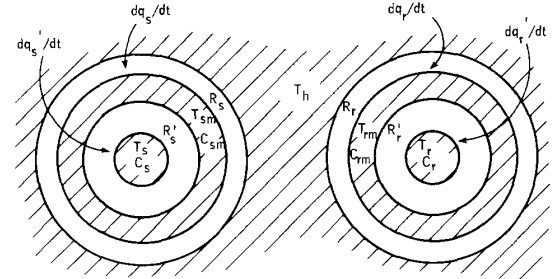
\includegraphics[width = 0.48\columnwidth]{/introduction/Mraw.png}
    \caption{Mraw のモデル\cite{Mraw}.
    左がサンプル試料、右側が参照用の試料の温度と熱抵抗の模式図になっている。}
    \label{fig:Mraw}
\end{wrapfigure}
DTA と DSC の動作原理として Mraw のモデル\cite{Mraw}がある(図\ref{fig:Mraw})。
これは DTA と DSC の測定装置をヒーターの温度、
温度計を取り付けることとなる試料側面、
試料のバルク部分に分け、
それぞれの間の熱流に関して微分方程式で説明する模型である。

図\ref{fig:Mraw} 右側のにある参照用の試料での熱の流れは
\begin{align}
    \dv{q_r}{t} = C_{rm}\dv{T_{rm}}{t}+C_r\dv{T_r}{t},\qquad
    \dv{q_r'}{t} = C_r \dv{T_r}{t}
\end{align}
というように表される。
ここでの \(\dv{q_r}{t}\) はヒーターから表面への熱流、
\(C_{rm}, C_{r}\) はそれぞれ表面部分とバルク部分の熱容量、
\(T_{rm}, T_{r}\) はそれぞれ表面部分とバルク部分の温度を表している。

一次相転移を起こさないときには左側にあるサンプル試料でも同様の式
\begin{align}
    \dv{q_s}{t} = C_{sm}\dv{T_{sm}}{t}+C_r\dv{T_s}{t}, \qquad
    \dv{q_s'}{t} = C_s \dv{T_s}{t}
\end{align}
で表される。
次に一次相転移が生じるときのことを考える。
試料表面ではその体積が小さくすぐに相転移が終わる。
バルク部分では一次相転移の潜熱のため温度は一定であり、
即座に潜熱分の熱が流入するわけではないので、
試料は転移が済んだ部分と済んでいない部分に分かれる。
これを微分方程式のモデルにすると、
\begin{align}
    \dv{q_s}{t} = C_{sm}\dv{T_{sm}}{t}+\Delta H\dv{\alpha}{t}, \qquad
    \dv{q_s'}{t} = \Delta H\dv{\alpha}{t}
\end{align}
というように表せる。
ここでの\(\Delta H\)は転移エンタルピー、
\(\alpha\)は試料中の転移が済んだ割合を表す。

熱流\(\dv{q}{t}\)は温度勾配に比例するというニュートンの冷却則
\begin{align}
    \dv{q}{t} = \frac{1}{R_r}(T_h-T_{rm})
\end{align}
を用いて温度としてあらわすことができるのでこれらの微分方程式を連立することで解くことができるのがわかる。

\begin{wrapfigure}{r}[0pt]{0.48\columnwidth}
    \centering
    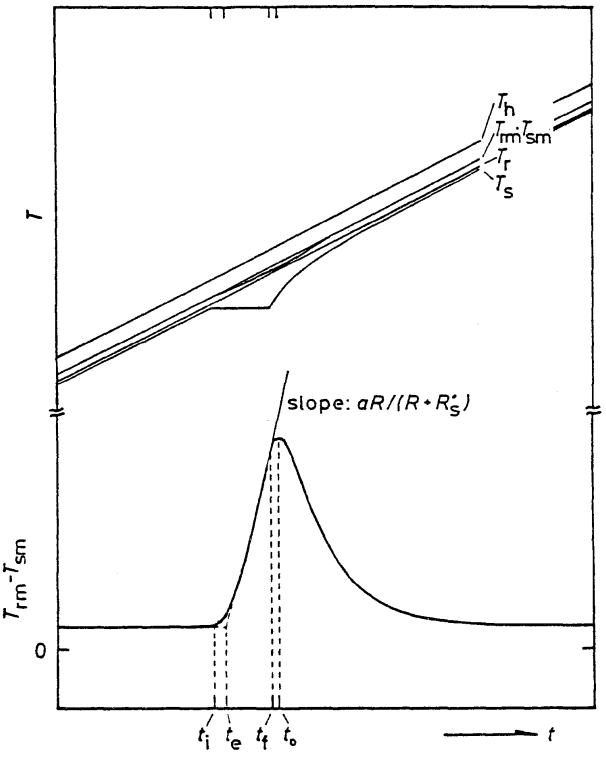
\includegraphics[width = 0.48\columnwidth]{/introduction/DSC.png}
    \caption{Mraw のモデルを使った一次相転移時の熱流束 DSC の振る舞い\cite{saito1987}.}
    \label{graph:theory}
\end{wrapfigure}
このモデルを DTA および DSC にどのように適用されるか見ていく。
古典的 DTA では試料表面で温度を測定するのではなく、内部の温度を測定する。
そのため始め表面部分と内部で分けていたが一体になったものとみなすことができ、
これらの間には熱抵抗は無く、\(T_{sm}=T_s,\,T_{rm}=T_r\)である。
そしてヒーターの温度は一定速度\(T_h=at+T_{h0}\)で変化するものとみなす。
この条件で微分方程式を解くとその振る舞いが得られる。
% TODO: appendix でちゃんと書きたいね
入力補償 DSC ではサンプル試料と参照用試料の表面での温度が同じになるように熱流を調整する。
そのため、ヒーター部分と表面部分が一体になったものとみなすことができる。
すると古典的 DTA と同じ式の形となるため入力補償 DSC で得られる温度のデータは古典的 DTA と同じような振る舞いとなる。

今回行う 熱流束 DSC ではそういった Mraw モデルのパラメータすべてを使うことになる。
このときヒーターと試料表面との間の熱抵抗は同じになるように装置は作ってある。
この熱抵抗を\(R=R_s=R_r\)とおく。
これを解析すると図\ref{graph:theory}のようになる\cite{saito1987}。
この図の縦軸に熱抵抗\(R\)を掛けることで熱流\(\dot{H}\)となるため、
これに温度を割ったものがエントロピー流\(\dot{S}\)となる。
また、相転移に伴う転移熱は相転移にかかわらないバックグラウンドを取り除いた熱流を考えればよい。
このバックグラウンドとして図\ref{graph:theory}の盛り上がった部分の下に引く線をベースラインと呼び、
ベースラインとピークに囲まれた領域の面積が転移エンタルピー\(\Delta H\), 転移エントロピー\(\Delta S\)となる。
そして比熱は
\begin{align}
    C_p = \qty(\pdv{H}{T})_p = \dv{t}{T}\dv{H}{t} = \frac{\dot{H}}{\dot{T}}
\end{align}
で求めることができる。

また、各手法とこの Mraw のモデルを考えると DTA と DSC は同じ測定原理・同じようなシグナルが出るという説明のされ方は不十分であるというのがわかる。
より正確には DTA と熱流束型 DSC は温度差を見るという点では同じ測定原理であるが、
シグナルは微分方程式モデルが異なることから違った形が出る、
DTA と入力補償型 DSC は測定原理は違うが、モデルは同じ形になるためシグナルは同じになると説明されるべきである。
\clearpage
\section{実験}
熱流型 DSC 測定機器である (株)日立ハイテクサイエンス DSC7020 を用いて、
In の固液相転移、Ni の磁気相転移、BTO の変異型強誘電相転移、TGS の秩序・無秩序型強誘電相転移に伴う熱異常を測定した。

\section{結果}
\subsection{数値微分}
比熱を計算する際に離散的なデータから微分を行う必要が生じる。
関数\(f(x)\)を微分する際に、微分を差分で近似する方法である
\begin{align}
    f'[i] = \frac{f[i+1]-f[i]}{x[i+1]-x[i]}
\end{align}
では分母の誤差が大きく出てしまうため、実際の微分とは大きくずれてしまうことが多い。
これを抑えるため、Savitzky-Golay フィルターを使った微分
\begin{align}
    f'[i] = \frac{86f[i-4]-142f[i-3]-193f[i-2]-126f[i-1]+126f[i+1]+193f[i+2]+142f[i+3]-86f[i+4]}{1188(x[i+1]-x[i])}
\end{align}
を使った。
また測定点が多いためこのフィルターを改良することができる。
連続するデータでは誤差に相関が生じるが、
離れれば離れるほど相関はなくなるため差分は離れた測定点同士で行うと誤差の影響が小さくなるので微分を
\begin{align}
    f'[i] = \frac{86f[i-40]-142f[i-30]-193f[i-20]-126f[i-10]+126f[i+10]+193f[i+20]+142f[i+30]-86f[i+40]}{1188( x[i+10]-x[i])}
\end{align}
というようにして計算をする。
\subsection{In の固体液相転移}
In の固液相転移付近における
熱流\(\dot{H}\), エントロピー流\(\dot{S}\), および比熱\(C_p\)は図\ref{graph:In}のようになった。
加熱時と冷却時で熱の流れの向きが逆になっているので符号が反転しているが同じようなシグナルとなっている。
また、相転移付近の温度とそれ以外の領域では流れの大きさが桁が違っていることから、
さらにゆっくり測定すると相転移では流れ・比熱ともに発散するのが予想される。
熱流\(\dot{H}\)とエントロピー流\(\dot{S}\)の間の関係は\(\dot{S}=\dot{H}/T\)であり、
温度が十分高いため図\ref{graph:In-current}ではスケールだけが違くて、
シグナルは同じ形となっている。
また、図\ref{graph:In-Cp}のグラフの立ち上がるところは温度計がある測定点で相転移が生じたことを表しているので、
転移温度の目安としてその値を読むと、加熱時と冷却時で違った温度になるのが確認できた。
これは一次相転移の過加熱・過冷却が生じていることを表している。
\begin{figure}[hbt]
    \centering
    \begin{minipage}[t]{0.52\columnwidth}
        \centering
        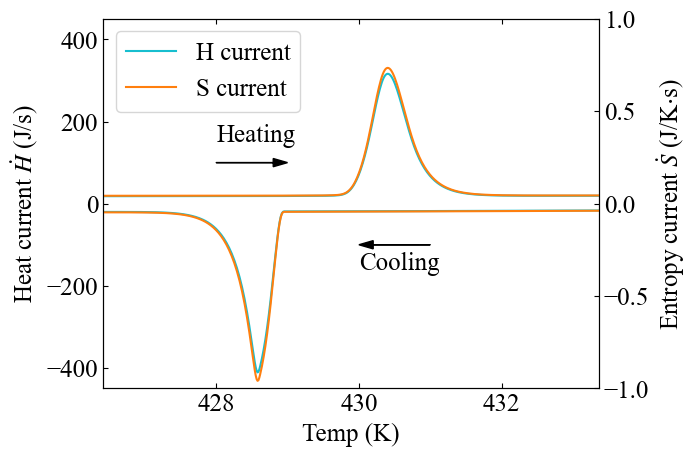
\includegraphics[width = \columnwidth]{result/In-current.png}
        \subcaption{熱流\(\dot{H}\), エントロピー流\(\dot{S}\)}
        \label{graph:In-current}
    \end{minipage}
    \hfill
    \begin{minipage}[t]{0.44\columnwidth}
        \centering
        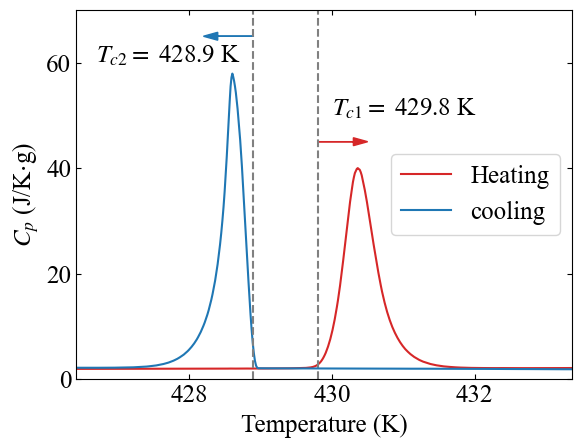
\includegraphics[width = \columnwidth]{result/In-Cp.png}
        \subcaption{比熱\(C_p\)}
        \label{graph:In-Cp}
    \end{minipage}
    \caption{相転移付近における In の熱的性質}
    \label{graph:In}
\end{figure}

\subsection{Ni の磁気相転移}
Ni の磁気相転移付近における熱流\(\dot{H}\), エントロピー流\(\dot{S}\), および比熱\(C_p\)は図\ref{graph:Ni}のようになった。
これは Mraw のモデルや図\ref{graph:In}で見たような一次相転移とは異なった熱異常となっている。
図\ref{graph:Ni-current}のスケールに注目すると相転移に伴って熱流が発散しないことから転移熱は小さいのがわかる。
そして相転移で比熱が発散せずに\(T_c = 630.4\) K で不連続に変わっているのが図\ref{graph:Ni-Cp}よりわかる。
この不連続になり始めた点を相転移点とする。
これよりは2次相転移であるとわかる。
また、加熱時と冷却時で比熱の値やその振る舞いは異なっているのがわかる。
\begin{figure}[hbt]
    \centering
    \begin{minipage}[t]{0.50\columnwidth}
        \centering
        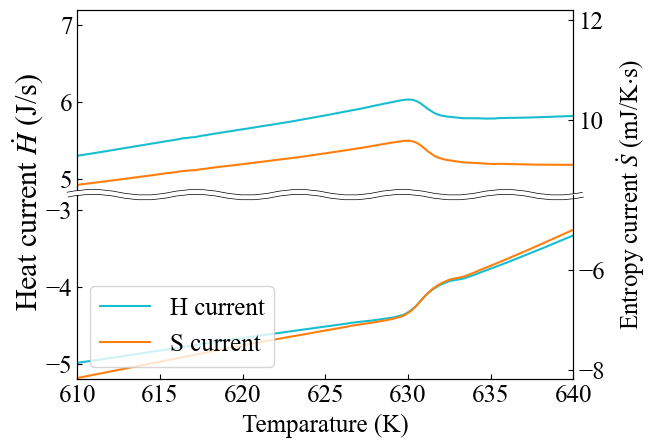
\includegraphics[width = \columnwidth]{result/Ni-current.png}
        \subcaption{熱流\(\dot{H}\), エントロピー流\(\dot{S}\)}
        \label{graph:Ni-current}
    \end{minipage}
    \hfill
    \begin{minipage}[t]{0.46\columnwidth}
        \centering
        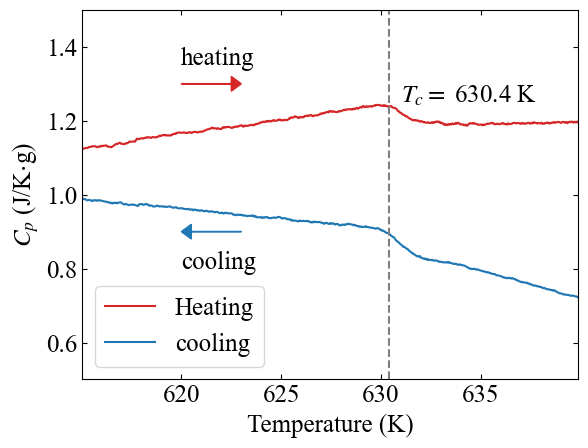
\includegraphics[width = \columnwidth]{result/Ni-Cp.png}
        \subcaption{比熱\(C_p\)}
        \label{graph:Ni-Cp}
    \end{minipage}
    \caption{相転移付近における Ni の熱的性質}
    \label{graph:Ni}
\end{figure}

\subsection{BTO の変異型強誘電相転移}
BTO の変異型強誘電相転移付近における熱流\(\dot{H}\), エントロピー流\(\dot{S}\), および比熱\(C_p\)は図\ref{graph:BTO}のようになった。
In の固液相転移と同じシグナルとなっていることから1次相転移になっているのがわかる。

ここで注目したいのが加熱時にはピークが2つある点である。
2つピークの形から読み取るとこれは BTO が正方晶から立方晶へと変化する際にほとんど同じ温度に2つの1次相転移の過程があり、
これは冷却する際には見れない現象となっている。
考えられる機構として分極のドメインの変化と結晶構造の変化というのがばらばらに見えているというのがある。
分極のドメインの変化は正方晶のa軸とc軸の入れかわりのような現象である。
格子定数は a = 6.9 \AA, c = 7.1 \AA とほとんど変わらないため昇温時の低い温度であっても起こりやすい。
一方、自発分極自体は結晶が正方晶でさえあればよいため、各ドメインは立方晶に代わるまで自発分極を持つ。
より、立方晶へと変化するのに必要な温度は高いと考えられる。
なので昇温時の2つのピークのうち低温側の小さいピークはドメインの変化によるもの、
高温側の大きいピークは正方晶から立方晶の変化によるものと考えられる。

降温時にはこの2つのピークが見れないのは昇温時とは違い、
立方晶から正方晶になると同時にドメインが生じるため、同じ温度で同時に起こることによるものであると考えられる。

\begin{figure}[hbt]
    \centering
    \begin{minipage}[t]{0.52\columnwidth}
        \centering
        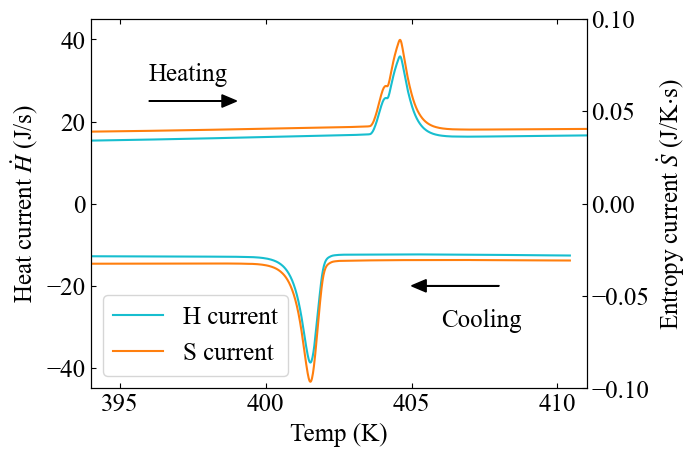
\includegraphics[width = \columnwidth]{result/BTO-current.png}
        \subcaption{熱流\(\dot{H}\), エントロピー流\(\dot{S}\)}
        \label{graph:BTO-current}
    \end{minipage}
    \hfill
    \begin{minipage}[t]{0.44\columnwidth}
        \centering
        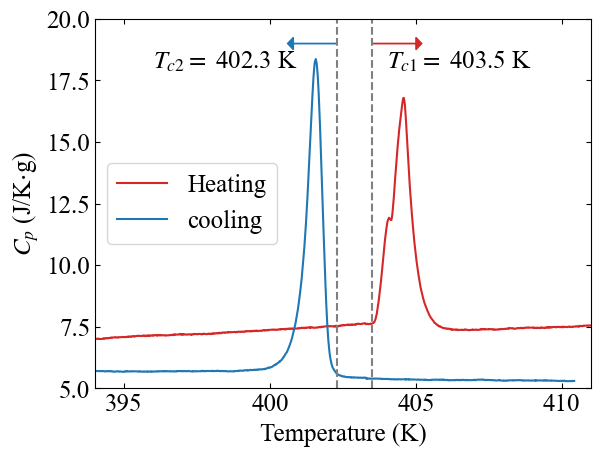
\includegraphics[width = \columnwidth]{result/BTO-Cp.png}
        \subcaption{比熱\(C_p\)}
        \label{graph:BTO-Cp}
    \end{minipage}
    \caption{相転移付近における BTO の熱的性質}
    \label{graph:BTO}
\end{figure}

\subsection{TGS の秩序・無秩序型強誘電相転移}
TGS の秩序・無秩序型強誘電相転移付近における熱流\(\dot{H}\), エントロピー流\(\dot{S}\), および比熱\(C_p\)は図\ref{graph:TGS}のようになった。
Ni の磁気相転移と同じシグナルとなっていることから2次相転移になっているのがわかる。

\begin{figure}[hbt]
    \centering
    \begin{minipage}[t]{0.51\columnwidth}
        \centering
        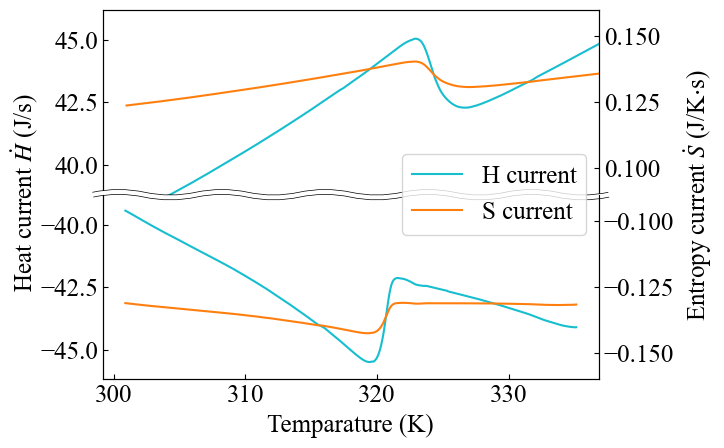
\includegraphics[width = \columnwidth]{result/TGS-current.png}
        \subcaption{熱流\(\dot{H}\), エントロピー流\(\dot{S}\)}
        \label{graph:TGS-current}
    \end{minipage}
    \hfill
    \begin{minipage}[t]{0.43\columnwidth}
        \centering
        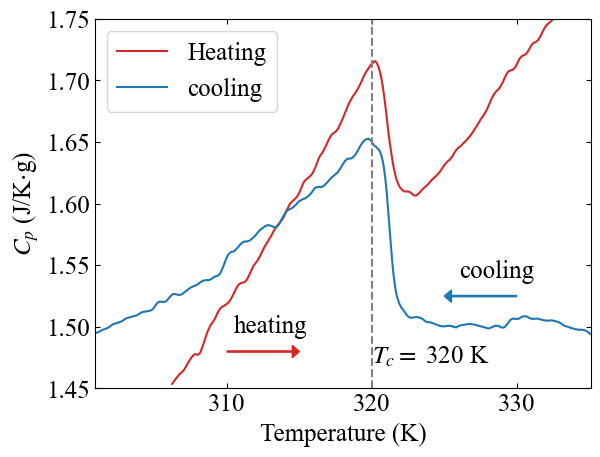
\includegraphics[width = \columnwidth]{result/TGS-Cp.png}
        \subcaption{比熱\(C_p\)}
        \label{graph:TSG-Cp}
    \end{minipage}
    \caption{相転移付近における TGS の熱的性質}
    \label{graph:TGS}
\end{figure}

\subsection{転移熱・転移エントロピー}
これら DSC 測定によって得られた熱流・エントロピー流のベースラインからのずれを積分することで
転移熱・転移エントロピーを求めることができる。
測定点が十分細かいため、数値積分を
\begin{align}
    \int f(x)dx = \sum_{i} f(x_i)\Delta x
\end{align}
というようにして行った。
この数値積分を実行すると各相転移の転移熱は表\ref{table:integral}のようになった。
積分を行った際のベースラインの取り方については appendix にまとめておいた。
\begin{table}[hbt]
    \centering
    \caption{各試料の相転移温度と転移熱・転移エントロピー}
    \label{table:integral}
    \begin{tabular}{lllll}
    \hline
                             & In    & Ni    & BTO   & TGS   \\
    \hline
    昇温時の転移温度 (K)       & 429.8 & 630.4 & 403.5 & 320.0 \\
    降温時の転移温度 (K)       & 428.9 & 630.4 & 402.3 & 320.0 \\
    昇温時の転移熱   (J/g)     & 2504  & 25.97 & 210.4 & 353.4 \\
    降温時の転移熱   (J/g)     & 2510  & 25.61 & 222.6 & 372.7 \\
    昇温時の転移エントロピー (mJ/K・g)   & 5819  & 41.26 & 520.1 & 1216  \\
    降温時の転移エントロピー (mJ/K・g)   & 5854  & 39.47 & 554.3 & 1187 \\
    \hline
    \end{tabular}
\end{table}

\clearpage
\section{考察}
\subsection{Rushbrooke の等式}
3OB 実験:強誘電性ヒステリシス曲線にて今回熱特性を測定した TGS と BTO の誘電特性を測定した。
違うサンプルではあるが、この実験では自発分極の温度特性と、常誘電相における D-E 特性の傾きから誘電率を調べることができる。
そのためスケーリング則の1つである Rushbrooke の等式

\begin{gather}
    \alpha + 2\beta +\gamma = 2\\
    C(T) \sim \frac{1}{\abs{T-T_c}^\alpha},\quad
    P(T) \sim (T_c-T)^\beta,\quad
    \chi(T) \sim \frac{1}{\abs{T-T_c}^\gamma}
\end{gather}
について確認ができる。
3OB 実験強誘電性ヒステリシス曲線の TGS と BTO の誘電特性の測定結果は図\ref{graph:TGS-histerisis},
図\ref{graph:BTO-histerisis} のようになった。
\begin{figure}[hbt]
    \centering
    \begin{minipage}[t]{0.48\columnwidth}
        \centering
        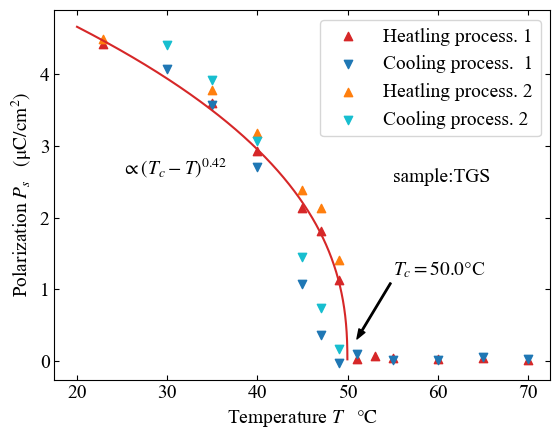
\includegraphics[width = \columnwidth]{discussion/TGS_Ps-T.png}
        \subcaption{自発分極}
        % \label{graph:TGS-current}
    \end{minipage}
    \hfill
    \begin{minipage}[t]{0.48\columnwidth}
        \centering
        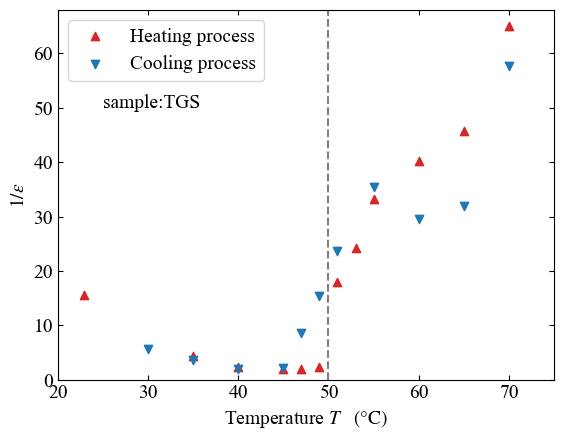
\includegraphics[width = \columnwidth]{discussion/TGS_epsilon1-T.png}
        \subcaption{誘電率}
        % \label{graph:TSG-Cp}
    \end{minipage}\\
    \caption{TGS の誘電特性。降温過程の測定はあまりに急速に冷却したためあまりうまくいっていない。}
    \label{graph:TGS-histerisis}

    \begin{minipage}[t]{0.48\columnwidth}
        \centering
        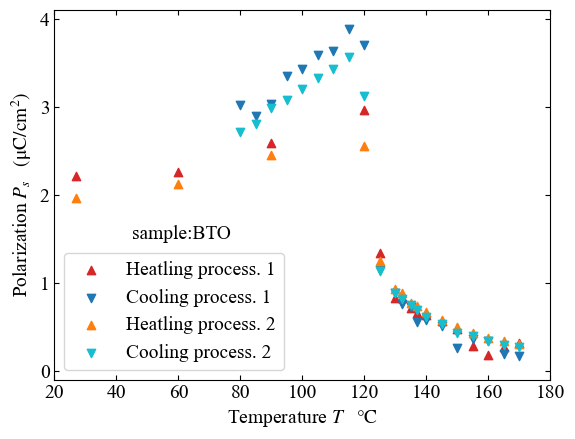
\includegraphics[width = \columnwidth]{discussion/BTO_Ps-T.png}
        \subcaption{自発分極}
        % \label{graph:TGS-current}
    \end{minipage}
    \hfill
    \begin{minipage}[t]{0.48\columnwidth}
        \centering
        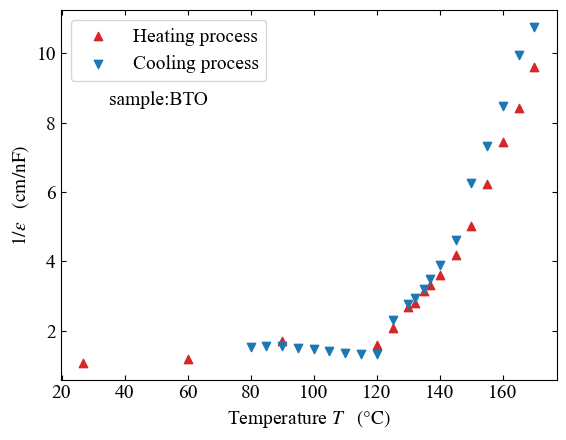
\includegraphics[width = \columnwidth]{discussion/BTO_epsilon-T1.png}
        \subcaption{誘電率}
        % \label{graph:TSG-Cp}
    \end{minipage}
    \caption{BTO の誘電特性}
    \label{graph:BTO-histerisis}
\end{figure}

まず TGS について臨界指数を読み取っていく。
まず比熱の発散の臨界指数 \(\alpha\) を見る。
図\ref{graph:TGS}では比熱の発散がなく、単なる飛びであるため、\(\alpha = 0\)とみなすことができる。
自発分極の臨界指数\(\beta\)は図\ref{graph:TGS-histerisis}より
\(\beta = 0.42\) であるとわかる。
また、誘電率の逆数がおおよそ温度に比例しているとみなすと \(\gamma=1\) とみなせる。
すると Rushbrooke の等式の左辺の値は
\begin{align}
    \alpha +2\beta+\gamma = 1.84
\end{align}
となり悪くない値が出てくる。
逆に Rushbrooke の等式が正しいとして、
測定のしにくい誘電率の冪を求めると \(\gamma = 1.16\) であるとわかる。

BTO の臨界指数について、図\ref{graph:BTO-histerisis} より自発分極の発散がないことから
\(\beta = 0\), 誘電率の発散は\(\gamma = 1\) とわかる。
これと Rushbrooke の等式より図\ref{graph:BTO-Cp}の比熱の発散は \(\alpha = 1\) であるとわかる。

\section{課題}
\begin{tcolorbox}[title = 課題1]
    \[\dot{Q}=C\dv{T}{t}\]を用いて
    \[H_Q-H_P = \int_{P\to Q}\dot{Q}dt\]
    および
    \[S_Q-S_P = \int_{P\to Q}\frac{\dot{Q}}{T}dt\]
    を示せ。
\end{tcolorbox}

\begin{align*}
    \int_{P\to Q}\dot{Q}dt
    = \int_{P\to Q} C\dv{T}{t}dt
    = \int_{P\to Q} \qty(\pdv{H}{T})_p dT
    = H_Q-H_P
\end{align*}
そして
\begin{align}
    \int_{P\to Q}\frac{\dot{Q}}{T}dt
    = \int_{P\to Q} \frac{C}{T}\dv{T}{t}dt
    = \int_{P\to Q} \qty(\pdv{S}{T})_p dT
    = S_Q-S_P
\end{align}

\begin{tcolorbox}[title = 課題2]
    4 つの試料について、昇温時と降温時の転移温度を比較し、
    異なっている場合にはその理由について考察せよ。
    なお、実験データから各試料について転移温度をどのように決定したかを明記せよ。
\end{tcolorbox}

結果のセクションで述べた。


\begin{tcolorbox}[title = 課題3]
    インジウムの融解熱(凝固熱)を調べ、実験で得られた転移エンタルピーと比較せよ。
\end{tcolorbox}

\cite{chem} の値を使うと In の融解熱は \(\Delta H = 28.58\) J/g である。
今回の測定で得られたものは\(\Delta H = 2504\) J/g, \(\Delta H = 2510\) J/g
というように近い値を得ることができた。

\section{結論}
熱異常の様子から In の固体液相転移は一次相転移、Ni の磁気相転移は二次相転移、
BTO の変異型強誘電は相転移一次相転移、TGS の秩序・無秩序型強誘電相転移は二次相転移であることが確認できた。
また、TGS では Rushbrooke の等式がおおよそ正しいことが確認できた。

% \clearpage
\bibliographystyle{junsrt}
\bibliography{reference}
\nocite{*}
\appendix
\section{転移熱を求める際のベースライン}
転移熱・転移エントロピーを求める際の相転移付近での Current の測定結果とそのベースライン、
積分値のグラフは以下の通りである。
\begin{figure}[hbt]
    \centering
    \begin{minipage}[t]{0.245\columnwidth}
        \centering
        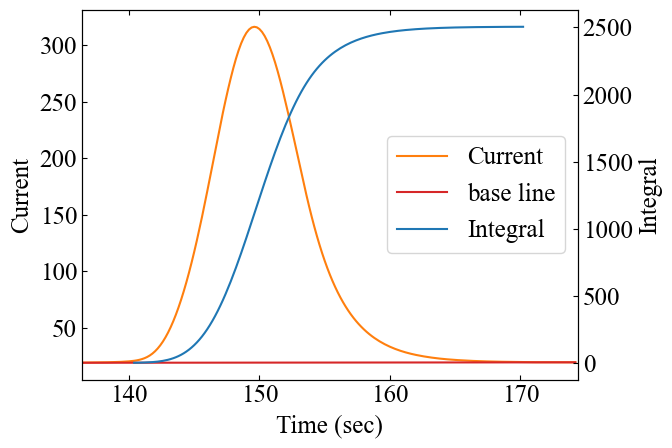
\includegraphics[width = \columnwidth]{appendix/In-dHdt-heat.png}
        \subcaption{\(\dot{H}\) heating}
    \end{minipage}
    \hfill
    \begin{minipage}[t]{0.245\columnwidth}
        \centering
        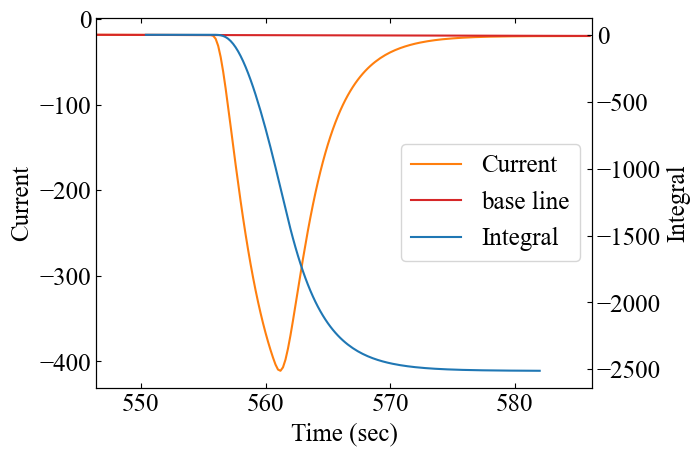
\includegraphics[width = \columnwidth]{appendix/In-dHdt-cool.png}
        \subcaption{\(\dot{H}\) cooling}
    \end{minipage}
    \hfill
    \begin{minipage}[t]{0.245\columnwidth}
        \centering
        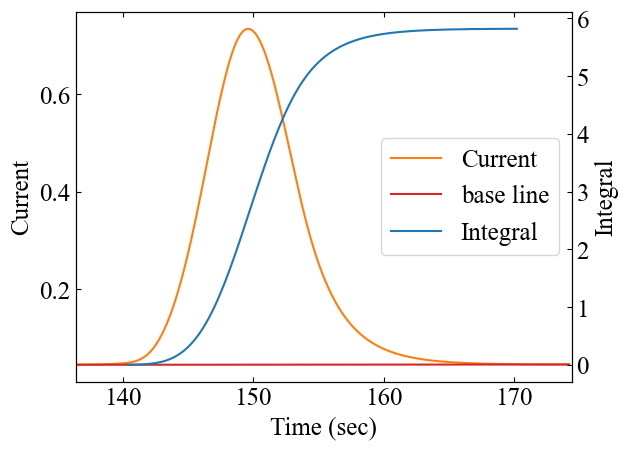
\includegraphics[width = \columnwidth]{appendix/In-dSdt-heat.png}
        \subcaption{\(\dot{S}\) heating}
    \end{minipage}
    \hfill
    \begin{minipage}[t]{0.245\columnwidth}
        \centering
        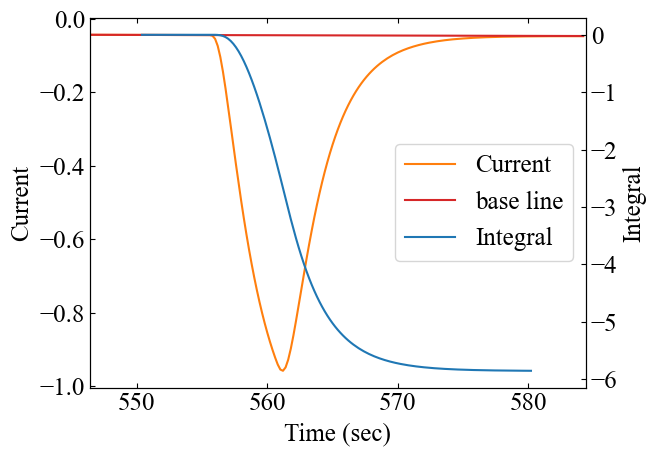
\includegraphics[width = \columnwidth]{appendix/In-dSdt-cool.png}
        \subcaption{\(\dot{S}\) cooling}
    \end{minipage}\\
    \caption{In}

    \begin{minipage}[t]{0.245\columnwidth}
        \centering
        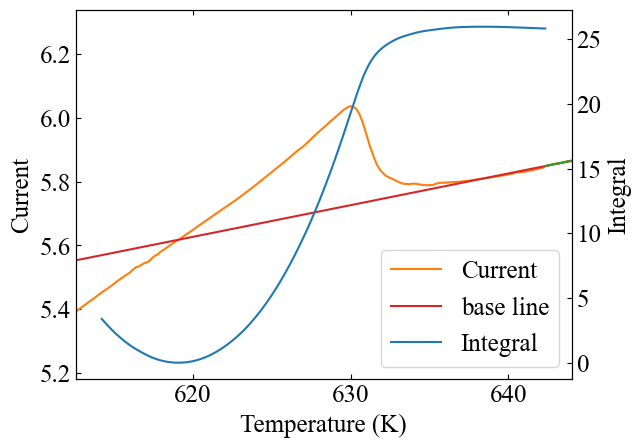
\includegraphics[width = \columnwidth]{appendix/Ni-dHdt-heat.png}
        \subcaption{\(\dot{H}\) heating}
    \end{minipage}
    \hfill
    \begin{minipage}[t]{0.245\columnwidth}
        \centering
        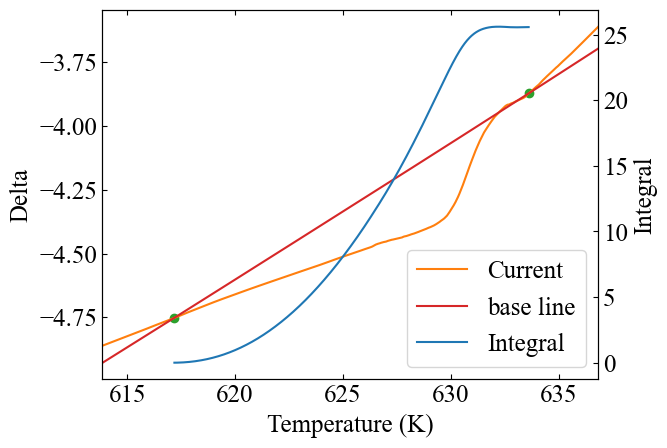
\includegraphics[width = \columnwidth]{appendix/Ni-dHdt-cool.png}
        \subcaption{\(\dot{H}\) cooling}
    \end{minipage}
    \hfill
    \begin{minipage}[t]{0.245\columnwidth}
        \centering
        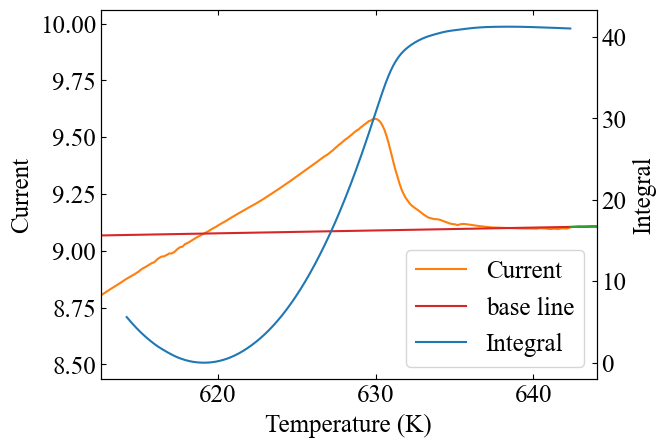
\includegraphics[width = \columnwidth]{appendix/Ni-dSdt-heat.png}
        \subcaption{\(\dot{S}\) heating}
    \end{minipage}
    \hfill
    \begin{minipage}[t]{0.245\columnwidth}
        \centering
        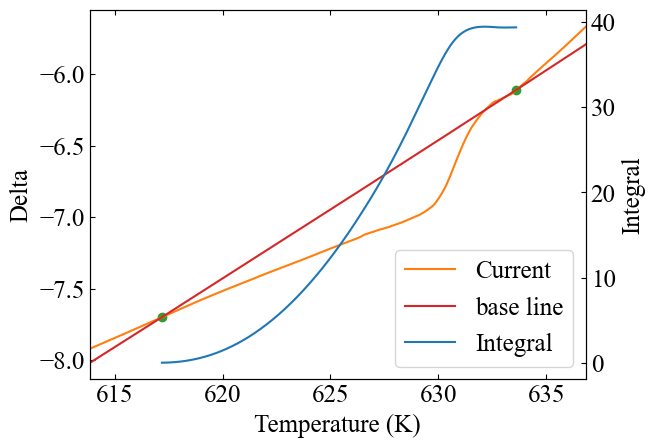
\includegraphics[width = \columnwidth]{appendix/Ni-dSdt-cool.png}
        \subcaption{\(\dot{S}\) cooling}
    \end{minipage}\\
    \caption{Ni}

    \begin{minipage}[t]{0.245\columnwidth}
        \centering
        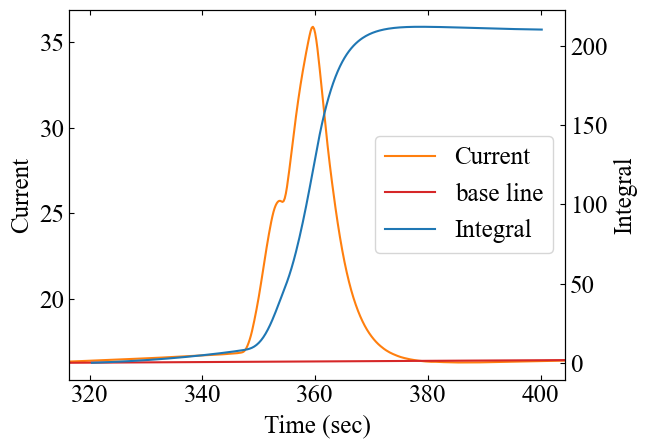
\includegraphics[width = \columnwidth]{appendix/BTO-dHdt-heat.png}
        \subcaption{\(\dot{H}\) heating}
    \end{minipage}
    \hfill
    \begin{minipage}[t]{0.245\columnwidth}
        \centering
        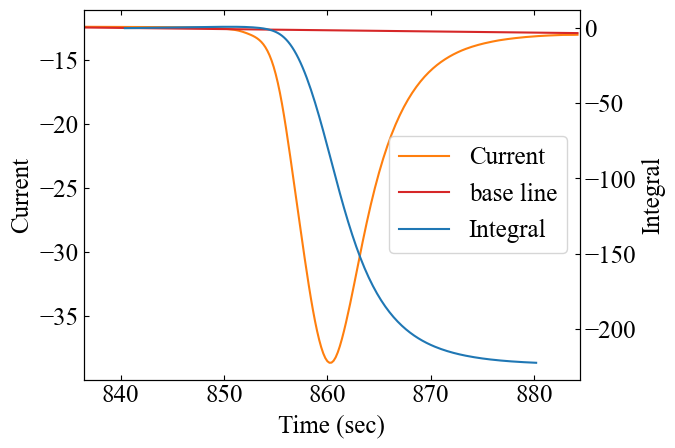
\includegraphics[width = \columnwidth]{appendix/BTO-dHdt-cool.png}
        \subcaption{\(\dot{H}\) cooling}
    \end{minipage}
    \hfill
    \begin{minipage}[t]{0.245\columnwidth}
        \centering
        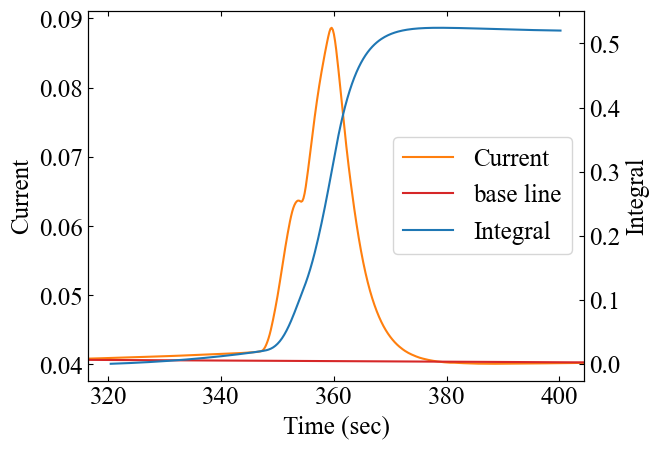
\includegraphics[width = \columnwidth]{appendix/BTO-dSdt-heat.png}
        \subcaption{\(\dot{S}\) heating}
    \end{minipage}
    \hfill
    \begin{minipage}[t]{0.245\columnwidth}
        \centering
        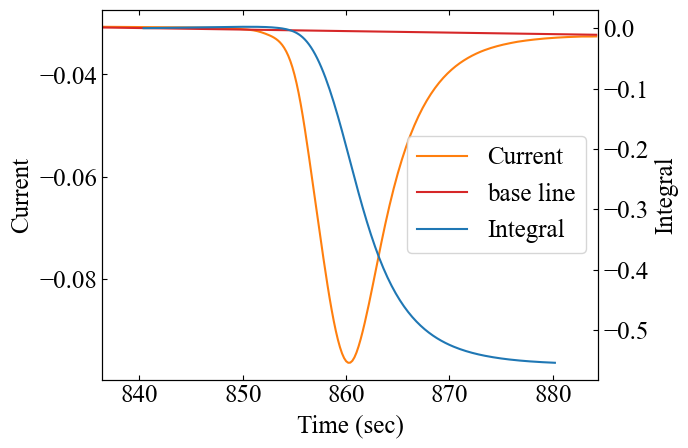
\includegraphics[width = \columnwidth]{appendix/BTO-dSdt-cool.png}
        \subcaption{\(\dot{S}\) cooling}
    \end{minipage}\\
    \caption{BTO}

    \begin{minipage}[t]{0.245\columnwidth}
        \centering
        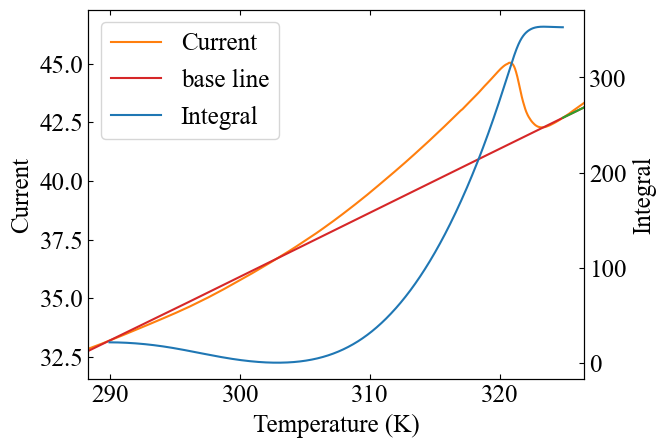
\includegraphics[width = \columnwidth]{appendix/TGS-dHdt-heat.png}
        \subcaption{\(\dot{H}\) heating}
    \end{minipage}
    \hfill
    \begin{minipage}[t]{0.245\columnwidth}
        \centering
        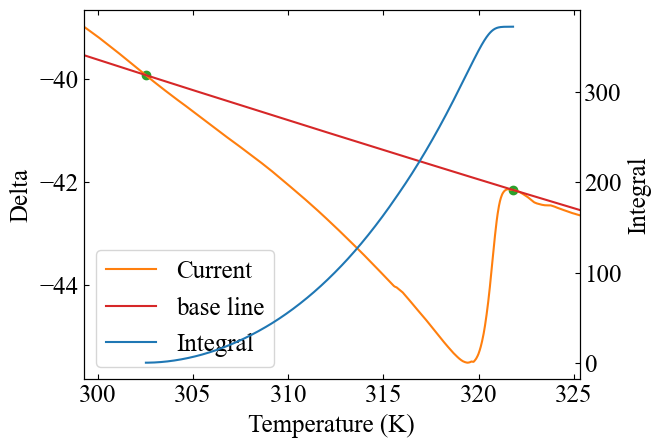
\includegraphics[width = \columnwidth]{appendix/TGS-dHdt-cool.png}
        \subcaption{\(\dot{H}\) cooling}
    \end{minipage}
    \hfill
    \begin{minipage}[t]{0.245\columnwidth}
        \centering
        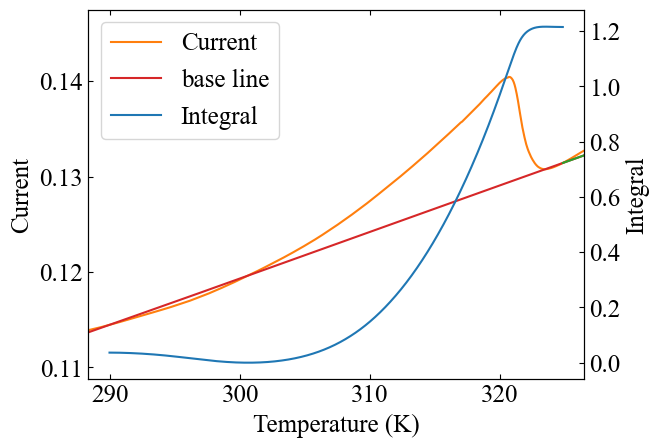
\includegraphics[width = \columnwidth]{appendix/TGS-dSdt-heat.png}
        \subcaption{\(\dot{S}\) heating}
    \end{minipage}
    \hfill
    \begin{minipage}[t]{0.245\columnwidth}
        \centering
        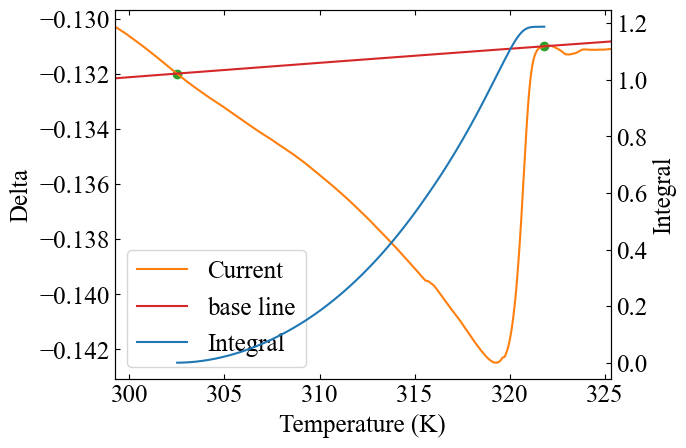
\includegraphics[width = \columnwidth]{appendix/TGS-dSdt-cool.png}
        \subcaption{\(\dot{S}\) cooling}
    \end{minipage}\\
    \caption{TGS}
\end{figure}

\end{document}